\chapter{Fase II: la Línea 3 como opción real}\label{cap:opciones}

\section{Planteamiento}

El análisis anterior supone que cada proyecto se construye en una fecha fija. Pero la decisión sobre la
Línea 3 no tiene por qué tomarse hoy: puede posponerse y tomarse con más información sobre la demanda.
Esa flexibilidad tiene valor, y la teoría de opciones reales permite medirlo.

Sea $d^-$ el diseño óptimo sin la Línea 3 (\OptimoNeutral) y $d^+$ el mismo diseño con la Línea 3
abierta. Para cada escenario se calcula el \emph{beneficio potencial} anual
\begin{equation}
B_t(\omega)=\big[C^{op}_t(d^-,\omega)-C^{op}_t(d^+,\omega)\big],
\end{equation}
la reducción del costo operativo (tiempo, auto y buses) que la línea produciría en el año $t$ si
estuviera abierta. Decidir en el año $\tau$ implica construir entre $\tau$ y $\tau+4$, abrir en
$\tau+5$, recibir $B_t$ desde entonces, pagar O\&M y recuperar el valor residual en 2050:
\begin{equation}\label{eq:vpn_tau}
\mathrm{VPN}_\tau(\omega)=\sum_{t\ge\tau+5}\delta_t\big(B_t(\omega)-\mathrm{O\&M}\big)
-\sum_{t=\tau}^{\tau+4}\delta_t\,\frac{I\,m(\omega)}{5}+\delta_{2050}\,R_\tau(\omega),
\end{equation}
con $m(\omega)$ el multiplicador de sobrecosto. Las fechas de decisión van de 2027 a 2040.

\section{Mínimos cuadrados de Monte Carlo}

A diferencia de una opción financiera, el valor de ejercer no se observa en la fecha de decisión,
porque depende de los beneficios futuros. Por eso se estiman por regresión tanto el valor de ejercer como
el de continuar, sobre un polinomio de grado 3 en la variable de estado observable, el beneficio
potencial corriente $B_\tau$:
\begin{enumerate}[nosep]
\item En la última fecha, ejercer si $\hat\E[\mathrm{VPN}_\tau\mid B_\tau]>0$.
\item Hacia atrás, en cada fecha $\tau$: estimar $\hat E_\tau(B)=\hat\E[\mathrm{VPN}_\tau\mid B_\tau]$ y
      la continuación $\hat C_\tau(B)=\hat\E[V_{\tau+1}\mid B_\tau]$; ejercer si
      $\hat E_\tau>\max(\hat C_\tau,0)$ y, en ese caso, asignar a la trayectoria su
      $\mathrm{VPN}_\tau$ realizado.
\item El valor de la opción es el promedio de los valores asignados (todos en valor presente de 2026).
\end{enumerate}
La \emph{frontera de ejercicio} en cada fecha es el menor beneficio potencial para el que conviene
decidir.

\section{Validación con McDonald y Siegel}

Antes de aplicarlo a la red, el algoritmo LSM se validó en el caso con solución cerrada
\eqref{eq:ms}: $V_0=I=1$, $\mu=2\,\%$, $\sigma=20\,\%$ y $r=6\,\%$, con 20.000 trayectorias antitéticas,
paso de 0,05 años y horizonte de 100 años. La solución analítica es $F(V_0)=\MSAnalitico$, con umbral
$V^*=\MSUmbral$ y $\beta=\MSBeta$; el LSM estima \MSLSM{} (error estándar \MSLSMEE), una diferencia de
\MSError. El sesgo hacia abajo es el esperado: la regla de ejercicio estimada por regresión es
subóptima y el ejercicio solo ocurre en fechas discretas, de modo que el LSM produce una cota inferior
del valor verdadero \citep{longstaff2001,glasserman2004}.

\section{Resultados}

La \cref{fig:opciones} resume la valoración. Comprometerse en 2027 a construir la Línea 3 tiene un VPN
esperado de \OpcionAhora{} billones: el ahorro operativo potencial de la línea, del orden de 2 a 3,5
billones anuales en la mediana, está lejos de cubrir la anualidad de una inversión de unos 46
billones con sobrecostos esperados. Posponer la decisión reduce la pérdida (el mejor año fijo dentro de la
ventana es \OpcionAnioEstatico, con \OpcionEstatico{} billones), pero sigue siendo negativo. La regla
flexible estimada por LSM vale \OpcionFlexible{} billones (error estándar \OpcionFlexibleEE): en el
\OpcionNunca{} de los escenarios la línea no se construye antes de 2040, y en el \OpcionEjerce{}
restante se construye cuando el ahorro potencial cruza una frontera de entre 8,4 y 9,5 billones
anuales.

\begin{figure}[ht]
\centering
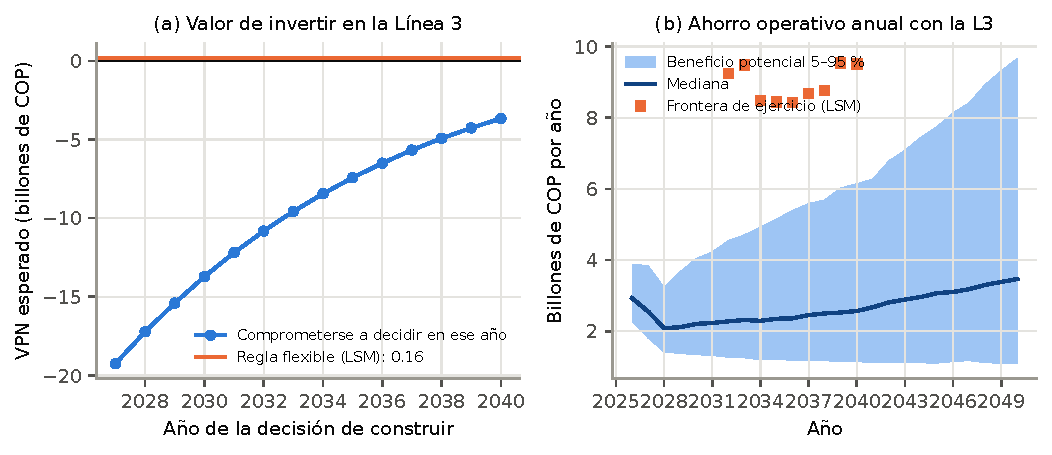
\includegraphics[width=\textwidth]{figuras/fig_opciones.pdf}
\caption{(a) VPN esperado de comprometerse a decidir en cada año y valor de la regla flexible.
(b) Beneficio potencial anual de la Línea 3 y frontera de ejercicio estimada.}\label{fig:opciones}
\end{figure}

La lectura correcta no es «la Línea 3 nunca debe construirse», sino que, con los supuestos centrales y
una tasa de 9\,\%, la información que justificaría construirla todavía no existe, y que la decisión
puede reducirse a vigilar un indicador observable: el ahorro de tiempo y de operación que la línea
produciría. Como mostró el \cref{cap:resultados}, una tasa de descuento menor o una mayor aversión a los
escenarios extremos acercan la frontera a la zona de ejercicio. Mientras tanto, conservar la opción
tiene un costo (reservar el corredor, avanzar en estudios y en gestión predial) que este modelo no
incluye y que debería compararse con el valor de la flexibilidad.
